\documentclass[12pt, a4paper]{article}

\usepackage[utf8]{inputenc}
\usepackage{geometry}
\geometry{top=1in, bottom=1in, left=1in, right=1in}
\usepackage{tikz}
\usetikzlibrary{shapes.geometric, arrows.meta, positioning, fit, backgrounds}

% TikZ Styles
\tikzstyle{process} = [rectangle, rounded corners, minimum width=3cm, minimum height=1cm, text centered, draw=black, fill=gray!10, text width=3.5cm]
\tikzstyle{database} = [cylinder, shape border rotate=90, aspect=0.25, draw, minimum height=2cm, minimum width=2.5cm, text centered, fill=blue!10]
\tikzstyle{arrow} = [thick, ->, >=stealth]
\tikzstyle{dashed_arrow} = [thick, ->, >=stealth, dashed]

\begin{document}

\begin{center}
    \textbf{\Large FORM 2} \\
    \textbf{THE PATENTS ACT, 1970 (39 of 1970)} \\
    \textbf{\&} \\
    \textbf{THE PATENTS RULES, 2003} \\
    \vspace{1cm}
    \textbf{\Large DRAWINGS FOR COMPLETE SPECIFICATION} \\
\end{center}

\vspace{1cm}
\noindent Applicant: Chirag Phogat, Chava Harshavardhan, Lalmalsawm Guite, Kaushal Pathak\\
\noindent Title: A DECOUPLED MULTI-PROCESS ARCHITECTURE FOR ASYNCHRONOUS SPATIAL AND ACOUSTIC HUMAN-COMPUTER INTERACTION

\newpage

% ================= FIGURE 1 =================
\begin{figure}[h!]
\centering
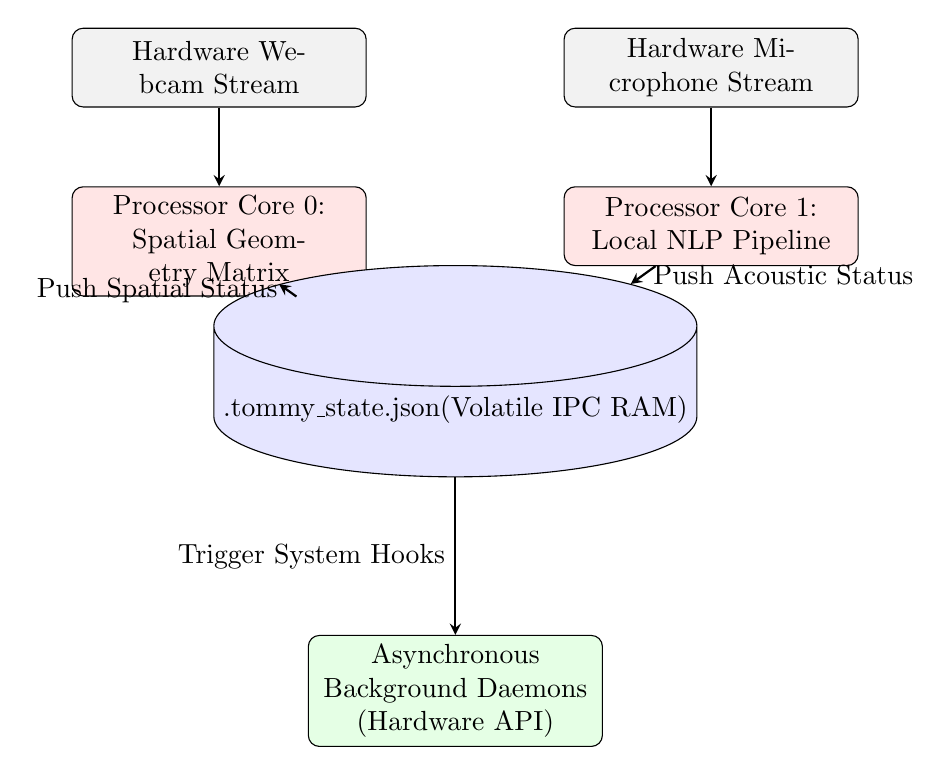
\begin{tikzpicture}[node distance=2.5cm]

    % Nodes
    \node (camera) [process] {Hardware Webcam Stream};
    \node (mic) [process, right=of camera] {Hardware Microphone Stream};
    
    \node (vision) [process, below=1cm of camera, fill=red!10] {Processor Core 0: \\ Spatial Geometry Matrix};
    \node (voice) [process, below=1cm of mic, fill=red!10] {Processor Core 1: \\ Local NLP Pipeline};
    
    \node (ipc) [database, below=2cm of camera, xshift=3cm] {.tommy\_state.json \\ (Volatile IPC RAM)};
    
    \node (daemon) [process, below=2cm of ipc, fill=green!10] {Asynchronous Background Daemons \\ (Hardware API)};
    
    % Arrows
    \draw [arrow] (camera) -- (vision);
    \draw [arrow] (mic) -- (voice);
    
    \draw [arrow] (vision) -- node[anchor=east] {Push Spatial Status} (ipc);
    \draw [arrow] (voice) -- node[anchor=west] {Push Acoustic Status} (ipc);
    
    \draw [arrow] (ipc) -- node[anchor=east] {Trigger System Hooks} (daemon);

\end{tikzpicture}
\vspace{1cm}
\caption{\textbf{FIG 1.} The decoupled multi-process architecture establishing separated IPC memory heaps across distinct CPU cores to eliminate interpreter locking.}
\end{figure}

\newpage

% ================= FIGURE 2 =================
\begin{figure}[h!]
\centering
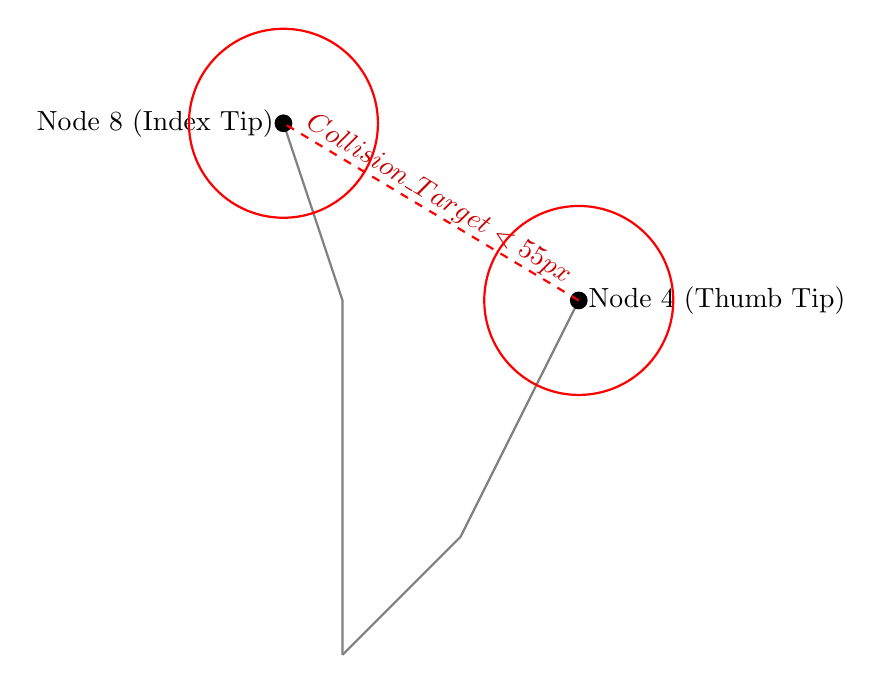
\begin{tikzpicture}[scale=1.5]

    % Points
    \coordinate (Base) at (0,0);
    \coordinate (Thumb1) at (1,1);
    \coordinate (Thumb2) at (1.5,2);
    \coordinate (ThumbTip) at (2,3); % Node 4
    
    \coordinate (Index1) at (0,1.5);
    \coordinate (Index2) at (0,3);
    \coordinate (IndexTip) at (-0.5,4.5); % Node 8

    % Lines
    \draw[thick, gray] (Base) -- (Thumb1) -- (Thumb2) -- (ThumbTip);
    \draw[thick, gray] (Base) -- (Index1) -- (Index2) -- (IndexTip);
    
    % Joint Nodes
    \filldraw[black] (ThumbTip) circle (2pt) node[anchor=west] {Node 4 (Thumb Tip)};
    \filldraw[black] (IndexTip) circle (2pt) node[anchor=east] {Node 8 (Index Tip)};
    
    % Bounding Box / Collision Parameter
    \draw[dashed, red, thick] (ThumbTip) -- (IndexTip) node[midway, above=-0.1cm, sloped, red!80!black] {$Collision\_Target < 55px$};
    
    % Radius boundary
    \draw[red, thick] (ThumbTip) circle (0.8cm);
    \draw[red, thick] (IndexTip) circle (0.8cm);

\end{tikzpicture}
\vspace{1cm}
\caption{\textbf{FIG 2.} Geometric collision zone mapping the exponential threshold bounding parameter ($<55px$) between Index-Node 4 and Thumb-Node 8 to eradicate physical Z-axis (depth) variations.}
\end{figure}

\newpage

% ================= FIGURE 3 =================
\begin{figure}[h!]
\centering
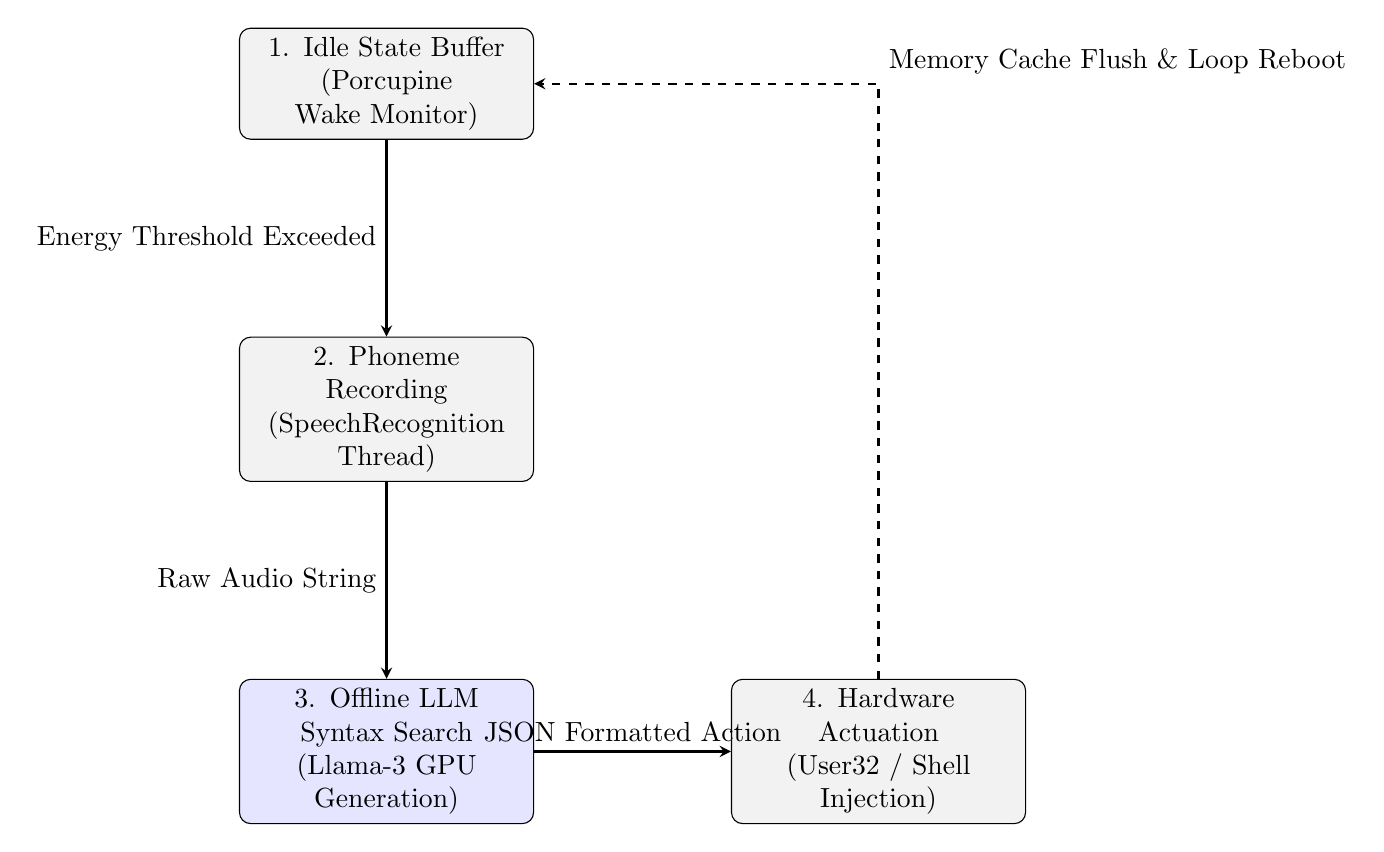
\begin{tikzpicture}[node distance=2.5cm]

    \node (idle) [process] {1. Idle State Buffer \\ (Porcupine Wake Monitor)};
    \node (record) [process, below=of idle] {2. Phoneme Recording \\ (SpeechRecognition Thread)};
    \node (llm) [process, below=of record, fill=blue!10] {3. Offline LLM Syntax Search \\ (Llama-3 GPU Generation)};
    \node (os) [process, right=of llm] {4. Hardware Actuation \\ (User32 / Shell Injection)};
    
    \draw [arrow] (idle) -- node[anchor=east] {Energy Threshold Exceeded} (record);
    \draw [arrow] (record) -- node[anchor=east] {Raw Audio String} (llm);
    \draw [arrow] (llm) -- node[anchor=south] {JSON Formatted Action} (os);
    
    % Recursive Arrow back to start
    \draw [dashed_arrow] (os) |- node[anchor=south west] {Memory Cache Flush \& Loop Reboot} (idle);

\end{tikzpicture}
\vspace{1cm}
\caption{\textbf{FIG 3.} The execution pipeline representing the recursive Local Host LLM logic ingestion bypassing native OS threading for completely offline auditory routing.}
\end{figure}

\end{document}
